\documentclass[11pt]{charter}

\usepackage{pgfgantt}
\usepackage[pdf]{pstricks}
\usepackage{pstricks}
\usepackage{tikz}
\usepackage{epsfig}
\usepackage{multicol}

% Central text tabla

\usepackage{array}
\newcolumntype{P}[1]{>{\centering\arraybackslash}p{#1}}
\newcolumntype{M}[1]{>{\centering\arraybackslash}m{#1}}

% Activity On Node

\usepackage[table]{xcolor}
\usepackage{array}

\definecolor{mygray}{RGB}{231,236,240}
\definecolor{myorange}{RGB}{253,205,148}
\definecolor{myblue}{RGB}{107,146,201}

\newcommand\ActTable[7]{%
  \begingroup
  \sffamily
  \renewcommand\arraystretch{1.5}%
  \begin{tabular}{*{3}{|>{\centering\arraybackslash}p{0.5cm}}|}
  \hline
  \rowcolor{mygray} #2 & #3 & #4 \\
  \hline
  \rowcolor{mygray}\multicolumn{3}{|c|}{Actividad #1} \\
  \hline
  \cellcolor{mygray}#5 & \cellcolor{myorange}\bfseries#6 & \cellcolor{mygray}#7 \\
  \hline
  \end{tabular}%
  \endgroup
}


% El títulos de la memoria, se usa en la carátula y se puede usar el cualquier lugar del documento con el comando \ttitle
\titulo{Implementación automatizada de redes neuronales para sistemas embebidos} 

% Nombre del posgrado, se usa en la carátula y se puede usar el cualquier lugar del documento con el comando \degreename
\posgrado{Carrera de Especialización en Sistemas Embebidos} 
%\posgrado{Carrera de Especialización en Internet de las Cosas} 
%\posgrado{Carrera de Especialización en Intelegencia Artificial}
%\posgrado{Maestría en Sistemas Embebidos} 
%\posgrado{Maestría en Internet de las cosas}

% Tu nombre, se puede usar el cualquier lugar del documento con el comando \authorname
\autor{Ing. José David Alvarado Moreno} 

% El nombre del director y co-director, se puede usar el cualquier lugar del documento con el comando \supname y \cosupname y \pertesupname y \pertecosupname
\director{Ing. Federico G. Zacchigna}
\pertenenciaDirector{FIUBA} 
% FIXME:NO IMPLEMENTADO EL CODIRECTOR ni su pertenencia
\codirector{} % si queda vacio no se deberíá incluir 
\pertenenciaCoDirector{}

% Nombre del cliente, quien va a aprobar los resultados del proyecto, se puede usar con el comando \clientename y \empclientename
\cliente{Ing. Federico G. Zacchigna}
\empresaCliente{FIUBA}

% Nombre y pertenencia de los jurados, se pueden usar el cualquier lugar del documento con el comando \jurunoname, \jurdosname y \jurtresname y \perteunoname, \pertedosname y \pertetresname.
\juradoUno{Nombre y Apellido (1)}
\pertenenciaJurUno{pertenencia (1)} 
\juradoDos{Nombre y Apellido (2)}
\pertenenciaJurDos{pertenencia (2)}
\juradoTres{Nombre y Apellido (3)}
\pertenenciaJurTres{pertenencia (3)}
 
\fechaINICIO{02 de marzo de 2021}		%Fecha de inicio de la cursada de GdP \fechaInicioName
\fechaFINALPlanificacion{22 de abril de 2021} 	%Fecha de final de cursada de GdP
\fechaFINALTrabajo{30 de noviembre de 2021}		%Fecha de defensa pública del trabajo final

\begin{document}

\maketitle
\thispagestyle{empty}
\pagebreak


\thispagestyle{empty}
{\setlength{\parskip}{0pt}
\tableofcontents{}
}
\pagebreak

\addcontentsline{toc}{section}{Registros de cambios}
\section*{Registros de cambios}
\label{sec:registro}


\begin{table}[ht]
\label{tab:registro}
\centering
\begin{tabularx}{\linewidth}{@{}|c|X|c|@{}}
\hline
\rowcolor[HTML]{C0C0C0} 
Revisión & \multicolumn{1}{c|}{\cellcolor[HTML]{C0C0C0}Detalles de los cambios realizados} 	& Fecha      \\ \hline
1.0      & Creación del documento                                          									& 02/03/2021 \\ \hline
1.1      & Avances ítems del 1 al 6	                                         								& 16/03/2021 \\ \hline
1.2      & Correcciones ítems del 1 al 6 e historias de usuarios 														& 23/03/2021 \\ \hline
1.3      & Correcciones ítems del 1 al 6 realizadas por el director 												& 30/03/2021 \\ \hline
1.4      & Correcciones ítems del 1 al 6 e historias de usuarios por el docente 						& 01/04/2021 \\ \hline
1.5      & Avances ítems del 6 al 11	 																											& 02/04/2021 \\ \hline
1.6      & Avances ítems del 12 al 17	 																											& 06/04/2021 \\ \hline
1.7      & Correcciones ítems del 6 al 17 													 												& 13/04/2021 \\ \hline

%					 Con texto partido \newline
%					 En varias líneas \newline
%					 A propósito                                                     									& dd/mm/aaaa \\ \hline
\end{tabularx}
\end{table}

\pagebreak

\addcontentsline{toc}{section}{Acta de constitución del proyecto}
\section*{Acta de constitución del proyecto}
\label{sec:acta}

\begin{flushright}
Buenos Aires, \fechaInicioName
\end{flushright}

\vspace{2cm}

Por medio de la presente se acuerda con el \authorname\hspace{1px} que su Trabajo Final de la \degreename\hspace{1px} se titulará ``\ttitle'', consistirá esencialmente en un prototipo preliminar de la implementación de redes neuronales convolucionales automatizadas, para reducir significativamente la complejidad y el tiempo que conlleva el codiseño de HW-SW, y tendrá un presupuesto preliminar estimado de 600 hs de trabajo y un costo de \$150 USD, con fecha de inicio \fechaInicioName\hspace{1px} y fecha de presentación pública \fechaFinalName.

Se adjunta a esta acta la planificación inicial.

\vfill

% Esta parte se construye sola con la información que hayan cargado en el preámbulo del documento y no debe modificarla
\begin{table}[ht]
\centering
\begin{tabular}{ccc}
\begin{tabular}[c]{@{}c@{}}Ariel Lutenberg \\ Director posgrado FIUBA\end{tabular} & \hspace{2cm} & \begin{tabular}[c]{@{}c@{}}\clientename \\ \empclientename \end{tabular} \vspace{2.5cm} \\ 
\multicolumn{3}{c}{\begin{tabular}[c]{@{}c@{}} \supname \\ Director del Trabajo Final\end{tabular}} \vspace{2.5cm} \\
%\begin{tabular}[c]{@{}c@{}}\jurunoname \\ Jurado del Trabajo Final\end{tabular}     &  & \begin{tabular}[c]{@{}c@{}}\jurdosname\\ Jurado del Trabajo Final\end{tabular}  \vspace{2.5cm}  \\
%\multicolumn{3}{c}{\begin{tabular}[c]{@{}c@{}} \jurtresname\\ Jurado del Trabajo Final\end{tabular}} \vspace{.5cm}                                                                     
\end{tabular}
\end{table}

\addcontentsline{toc}{section}{Descripción técnica-conceptual del proyecto a realizar}
\section*{Descripción técnica-conceptual del proyecto a realizar}
\label{sec:descripción}

En la actualidad encontramos diferentes aplicaciones de inteligencia artificial que utilizan redes neuronales (RN). Para este tipo de desarrollos generalmente se requiere procesar un alto volumen de información por lo que es necesario que los dispositivos a utilizar incorporen una gran capacidad de procesamiento y almacenamiento, para lo cual se puede encontrar con diferentes alternativas de sistemas embebidos en donde es posible realizar esta implementación como por ejemplo: MCU, GPU, FPGA, DLP y ASIC. Al evaluar cada uno en términos de desempeño, flexibilidad y capacidad de integración en un sistema embebido (SE) encontramos que los MCU y ASIC presentan una baja \textit{performance}; las GPU presentan baja capacidad de integración y los DLP presentan una flexibilidad para aplicaciones especificas; y por último encontramos que las FPGA presentan una alta flexibilidad, aunque muchas veces se ve opacada por la complejidad que conlleva el desarrollo del sistema. 

El proyecto general busca el desarrollo de un software (SW) para la implementación del algoritmo de clasificación de una Red Neuronal (RN) de manera automatizada a partir de un modelo de alto nivel  y que incorpore una interfaz necesaria para acceder, controlar y monitorear su funcionamiento desde un microcontrolador de propósito general. para lo cual se utilizará una SOC-FPGA en el cual coexisten un microprocesador de propósito general y un bloque de hardware (HW) dedicado exclusivamente a realizar el procesamiento de datos asociado a la RN, cuyo fin es el de liberar al microprocesador de estas tareas. Al diseño de este tipo de arquitecturas se lo conoce como “codiseño de HW-SW”. En la Figura \ref{fig:diagBloques} se muestra un diagrama en bloques simplificado del sistema.          

\vspace{25px}

\begin{figure}[htpb]
\centering 
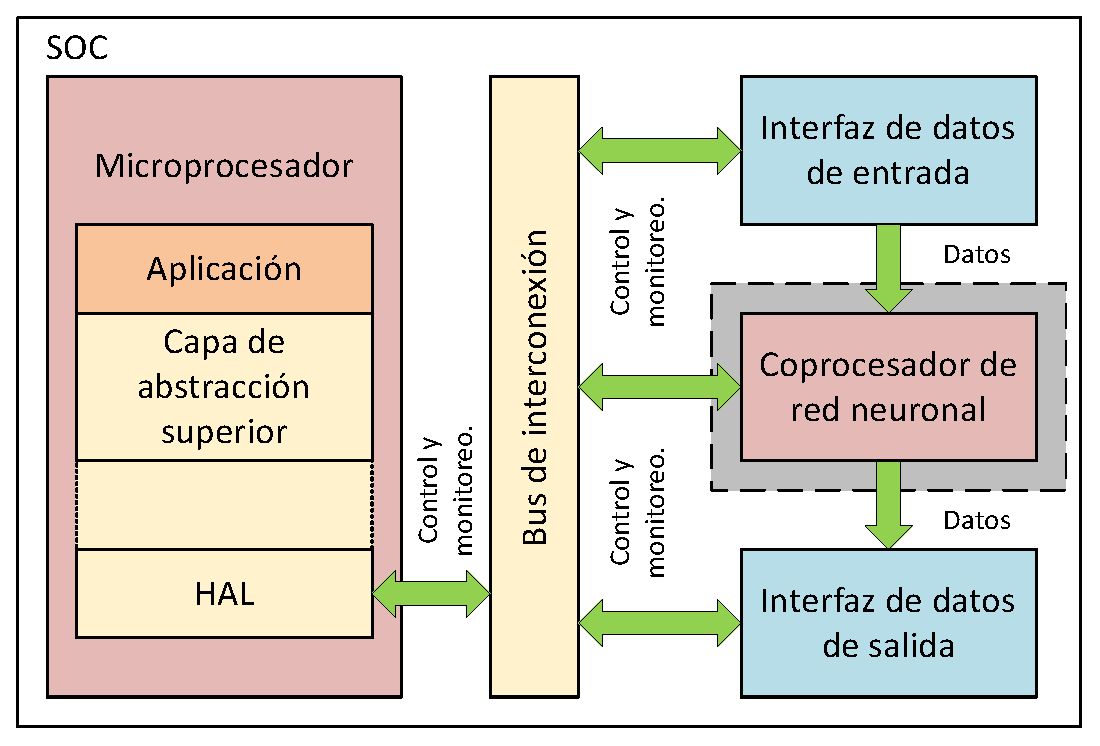
\includegraphics[width=.7\textwidth]{./Figuras/Diagramas.eps}
\caption{Diagrama en bloques del sistema}
\label{fig:diagBloques}
\end{figure}

\vspace{25px}

En este proyecto se realizará específicamente el bloque de hardware en la FPGA denominado \textit{\textbf{coprocesador de red neuronal}} (bloque resaltado en color gris de la Figura \ref{fig:diagBloques}), para un modelo de red neuronal convolucional (RNC). En la Figura \ref{fig:RN1} se presenta el modelo de una RNC, en donde se pueden identificar las diferentes etapas para el proceso de clasificación. En este tipo de RNC las etapas de convolución y \textit{subsampling} se pueden realizar en varias veces en las diferentes capas dependiendo del modelo diseñado, y lo que se busca con el sistema propuesto de red automatizada es que sea posible ajustar el número y el tamaño de las diferentes capas internas de la red como se muestra en la Figura \ref{fig:RN2}.          

\vspace{25px}

\begin{figure}[htpb]
\centering 
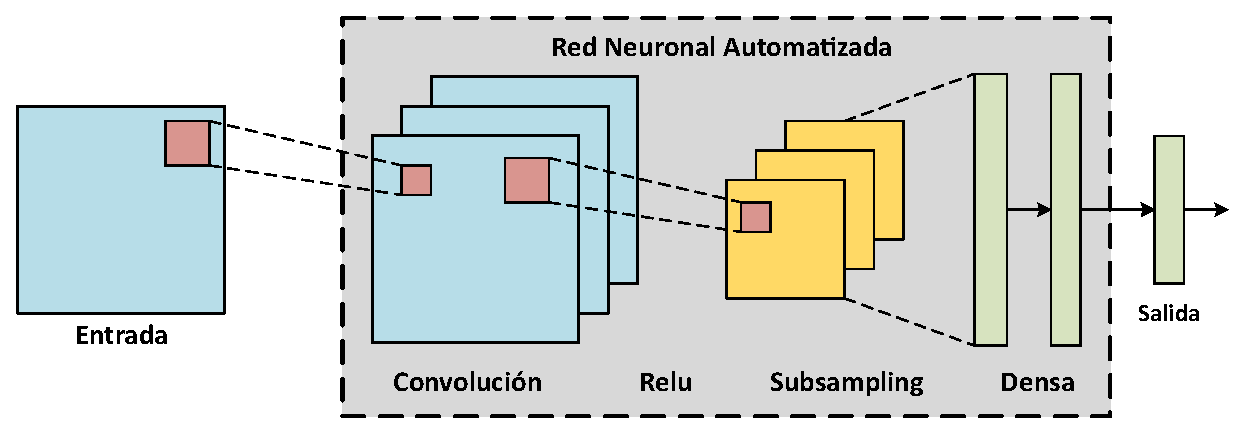
\includegraphics[width=.9\textwidth]{./Figuras/RN1.eps}
\caption{Diagrama en bloques red neuronal convolucional}
\label{fig:RN1}
\end{figure}

\vspace{25px}

\begin{figure}[htpb]
\centering 
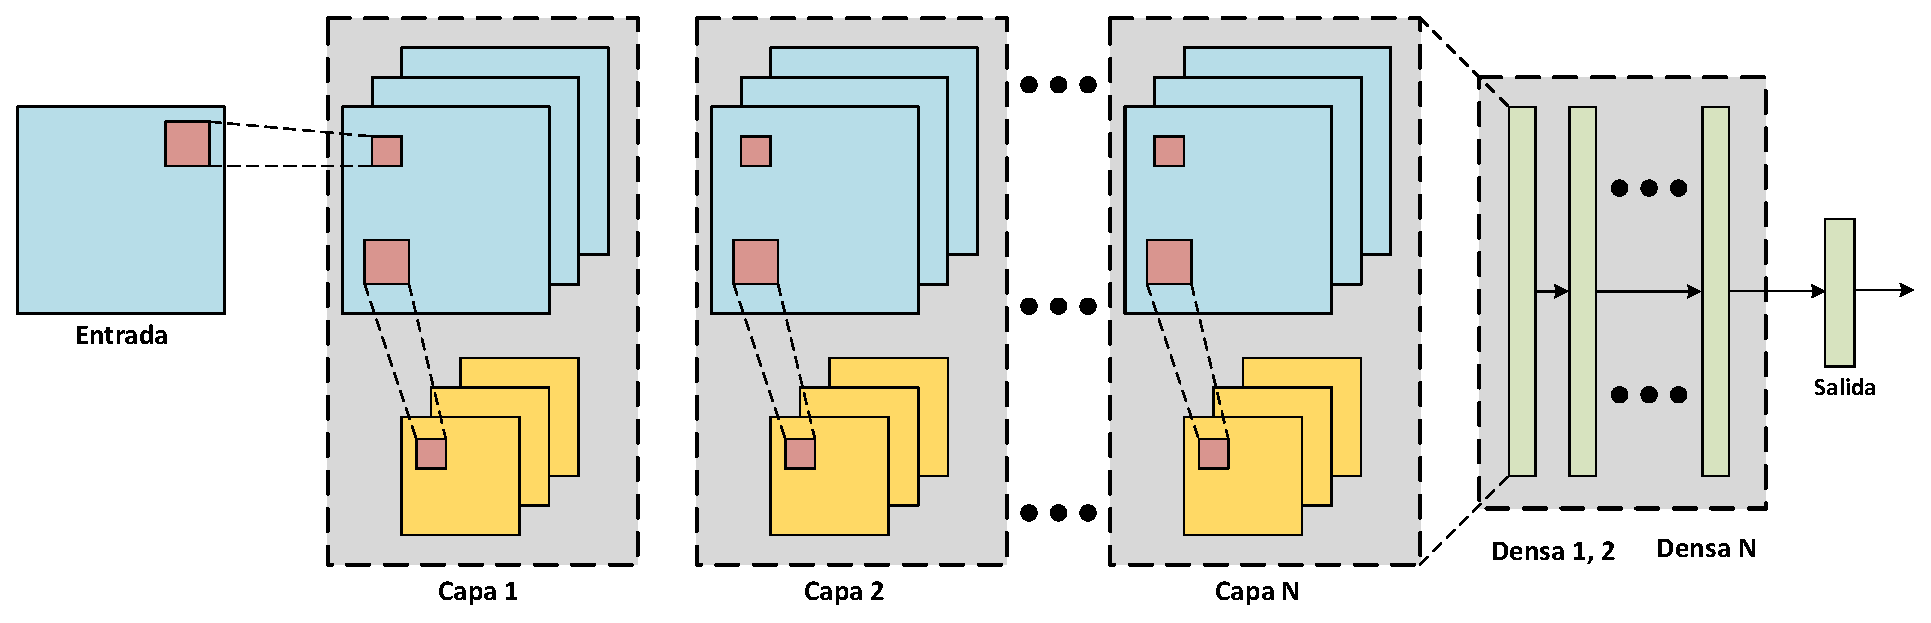
\includegraphics[width=.99\textwidth]{./Figuras/RN2.eps}
\caption{Diagrama en bloques red neuronal automatizada}
\label{fig:RN2}
\end{figure}

\vspace{25px}

Este trabajo tiene como objetivo principal reducir significativamente la complejidad y el tiempo que conlleva el codiseño de HW-SW e implementación de una RN en una SoC-FPGA y de esta manera eliminar una de las grandes barreras para su utilización.

\addcontentsline{toc}{section}{Identificación y análisis de los interesados}
\section*{Identificación y análisis de los interesados}
\label{sec:interesados}

\begin{table}[ht]
%\caption{Identificación de los interesados}
%\label{tab:interesados}
\begin{tabularx}{\linewidth}{@{}|l|X|X|l|@{}}
\hline
\rowcolor[HTML]{C0C0C0} 
Rol           & Nombre y Apellido & Organización 		& Puesto 								 \\ \hline
%Auspiciante   &                   &              		& -      								 \\ \hline
Cliente       & \clientename      &\empclientename	& -      								 \\ \hline
%Impulsor      &                   &              		& -      								 \\ \hline
Responsable   & \authorname       & FIUBA        		& Alumno 								 \\ \hline
%Colaboradores & -                 & -            		& -      								 \\ \hline
Orientador    & \supname	    	  & \pertesupname 	& Director Trabajo final \\ \hline
%Equipo        & -           			& -            		& -      								 \\ \hline
%Opositores    & -                 & -            		& -      								 \\ \hline
%Usuario final & -                 & -            		& -      								 \\ \hline
\end{tabularx}
\end{table}

\addcontentsline{toc}{section}{1. Propósito del proyecto}
\section*{1. Propósito del proyecto}
\label{sec:proposito}

El propósito de este proyecto es el desarrollo de un módulo de hardware para un coprocesador de red neuronal a partir de un modelo de alto nivel, en el cual se implementarán todas las capas de la red neuronal (RN), \textit{subsampling} y clasificación de la RN, en donde sea posible ajustar la arquitectura de la RNC a partir de los parámetros definidos por el tamaño de los datos de entrada y las características definidas de la arquitectura para el número de capas de la RN. 

\addcontentsline{toc}{section}{2. Alcance del proyecto}
\section*{2. Alcance del proyecto}
\label{sec:alcance}

En el presente proyecto se realizaran las siguientes actividades:

\begin{itemize}
	\item Establecer el modelo de alto nivel de red neuronal utilizando una herramienta de software especializada.    
	%\item Definir los parámetros adecuados para realizar cuantización. 
	\item Diseñar e implementar la arquitectura de alto nivel y la la micro-arquitectura de cada uno de los módulos internos.
	\item Implementar el modelo de red neuronal automatizada  utilizando lenguaje de alto nivel.
	\item Verificación y validación del funcionamiento del sistema.
	\item Realizar la documentación del trabajo final. 
\end{itemize}

El presente proyecto no incluye realizar procesos de optimización en las etapas de cuantización y arquitectura de alto de nivel, adicionalmente no se complementará con dispositivos para realizar la captura o para la visualización de los patrones. Por último, no se realizarán desarrollos de hardware o incorporación de periféricos externos a los que están en la placa   PYNQ-Z2.

% Definir los parámetros y características de los patrones de entrada de la red neuronal.

\addcontentsline{toc}{section}{3. Supuestos del proyecto}
\section*{3. Supuestos del proyecto}
\label{sec:supuestos}

Para el desarrollo de este proyecto se supone que es posible implementar las diferentes capas de la RNC en la placa TUL PYNQ-Z2 (ZYNQ XC7Z020-1CLG400C), y con la herramienta de software Vivado HLx versión webpack.

\addcontentsline{toc}{section}{4. Requerimientos}
\section*{4. Requerimientos}
\label{sec:requerimientos}

\begin{enumerate}

\item Requerimientos funcionales etapa de convolución. 
	\begin{enumerate}
	\item La herramienta debe permitir que los datos de entrada y salida en la capa de convolución se realicen por medio de un interfaz de \textit{streaming} de datos. 
	\item La herramienta debe permitir cargar los valores de los pesos y el tamaño del kernel.
	\item El sistema debe realizar la convolución para procesar la información de la capa anterior.
	\end{enumerate}

\item Requerimientos funcionales etapa de \textit{subsampling}. 
	\begin{enumerate}
	\item La herramienta debe permitir que los datos de entrada y salida en la capa de \textit{subsampling} se realicen por medio de un interfaz \textit{streaming} de datos. 
	\item La herramienta debe permitir seleccionar el método de \textit{subsampling}.
	\item El sistema debe realizar la \textit{subsampling} para procesar la información de la capa anterior.
	\end{enumerate}

\item Requerimientos funcionales etapa de clasificación (Capa densa). 
	\begin{enumerate}
	\item La herramienta debe permitir que los datos de entrada y salida en la capa de densa se realicen por medio de un interfaz de \textit{streaming} de datos. 
	\item El sistema debe realizar la clasificación para procesar la información de la capa anterior.
	\end{enumerate}

\item Requerimientos funcionales de software. 
	\begin{enumerate}
	\item La herramienta debe tomar como entrada un modelo de una red neuronal de alto nivel (Keras).
	%\item La herramienta debe generar un modelo cuantizado para VHDL.
	\item La herramienta debe generar un modelo de la arquitectura digital del alto nivel.
	\item La herramienta debe generar un modelo de la arquitectura de alto nivel a partir del modelo cuantizado.
	\item La herramienta debe generar una \textit{Golden Reference} (GR) a partir de la arquitectura de alto nivel.
	\item La herramienta debe generar el código HDL sintetizable a partir de la arquitectura de alto nivel.
	\item La herramienta debe generar un \textit{testbench} de simulación, que permita comparar los resultados de HW con los resultados de la GR.
	\end{enumerate}

\item Requerimientos funcionales del código HDL generado. 
	\begin{enumerate}
	\item El sistema debe presentar un funcionamiento equivalente al modelo cuantizado.
	\item El sistema debe utilizar un número de multiplicadores fijo por cada etapa de acuerdo a la arquitectura de alto nivel.
	%\item La herramienta debe permitir que las interfaces de entrada y salida sean de \textit{streaming} de datos.
	\item El sistema debe ser configurado, controlado y monitoreado a través de un banco de registros.
	\end{enumerate}

\item Requerimientos documentales. 
	\begin{enumerate}
	
	\item Se debe realizar el documento de informe de avance.
	\item Se debe realizar el documento de informe final.
	%\item Se debe realizar el documento del SW de generación automática.
	%\item Se debe realizar el documento del módulo generado automáticamente.
	\end{enumerate}

\end{enumerate}

\addcontentsline{toc}{section}{Historias de usuarios (\textit{Product backlog})}
\section*{Historias de usuarios (\textit{Product backlog})}
\label{sec:backlog}

%Como usuario, quiero que se posible especificar las características, tamaño y el tipo de los datos de entrada.
%Como usuario, quiero que se posible definir el tamaño del kernel 3x3 o 5x5 para la capa de convolución. 
%Como usuario, quiero que se posible definir el numero de capas de convolución. 
%Como usuario, quiero que se posible definir el numero de capas y el método de \textit{subsampling}. 
%Como usuario, quiero que se posible definir el numero de capas densa. 

%A continuación, se encuentran las historias de usuario y su ponderación calculada en story point ([0.5] al [100])

A continuación, se encuentran las historias de usuario:

\begin{itemize}
	\item Como usuario he diseñado y entrenado una RN utilizando Keras y quiero migrarla a un sistema embebido.. % [3] 
	\item Como usuario quiero explorar distintas estrategias de cuantización de una RN y relevar el impacto en la utilización de recursos al implementarla en una FPGA. % [2] 
	\item Como usuario quiero explorar distintas arquitecturas de RN para su implementación en FPGA y evaluar el rendimiento y la utilización de recursos en cada caso. % [2] 
	\item Como usuario quiero realizar pruebas de campo de RN implementadas en un sistema embebido para evaluar su rendimiento en un ambiente real. % [2] 
\end{itemize}

\addcontentsline{toc}{section}{5. Entregables principales del proyecto}
\section*{5. Entregables principales del proyecto}
\label{sec:entregables}

\begin{itemize}
\item Plan de trabajo del proyecto.
\item SW de generación automática del código VHLD.
\item Documento del SW de generación automática.
\item Documento del módulo generado automáticamente.
\item Documento de informe de avance.
\item Documento de informe final.
\end{itemize}

\addcontentsline{toc}{section}{6. Desglose del trabajo en tareas}
\section*{6. Desglose del trabajo en tareas}
\label{sec:wbs}

A continuación se presenta el desglose de las actividades y la duración estimada para el desarrollo del proyecto. 

\begin{enumerate}
\item Planificación general del proyecto.
	\begin{enumerate}
	\item \begin{tabular}[]{p{11cm} p{2cm}} Elaboración del plan de trabajo del proyecto 	& 30 hs \end{tabular}
	\item \begin{tabular}[]{p{11cm} p{2cm}} Planificación del proyecto  									& 10 hs \end{tabular}
	\end{enumerate}
\item Revisión bibliográfica y especificaciones. 
	\begin{enumerate}
	\item \begin{tabular}[]{p{11cm} p{2cm}} Revisión de la bibliografía específica   			& 40 hs \end{tabular}
	\item \begin{tabular}[]{p{11cm} p{2cm}} Especificación de requisitos  								& 20 hs \end{tabular}
	\item \begin{tabular}[]{p{11cm} p{2cm}} Definición de los casos de uso 								& 20 hs \end{tabular}
	\end{enumerate}
\item Desarrollo de red neuronal automatizada.  
	\begin{enumerate}
	\item \begin{tabular}[]{p{11cm} p{2cm}} Desarrollo del algoritmo de ventaneo			 											& 30 hs \end{tabular}
	\item \begin{tabular}[]{p{11cm} p{2cm}} Desarrollo del algoritmo de convolución  												& 60 hs \end{tabular}
	\item \begin{tabular}[]{p{11cm} p{2cm}} Desarrollo del algoritmo de \textit{subsampling} 								& 40 hs \end{tabular}
	\item \begin{tabular}[]{p{11cm} p{2cm}} Desarrollo de las unidades de control    												& 40 hs \end{tabular}
	\item \begin{tabular}[]{p{11cm} p{2cm}} Desarrollo del algoritmo de clasificación   										& 60 hs \end{tabular}
	\item \begin{tabular}[]{p{11cm} p{2cm}} Desarrollo del sistema de integración de la arquitectura    		& 60 hs \end{tabular}
	\end{enumerate}
\item Verificación y validación.
	\begin{enumerate}
	\item \begin{tabular}[]{p{11cm} p{2cm}} Pruebas de las capas: convolución, \textit{subsampling} y densa.											& 20 hs \end{tabular}
	\item \begin{tabular}[]{p{11cm} p{2cm}} Pruebas integrales del sistema y validación completa del proceso de automatización 		& 20 hs \end{tabular}
	\item \begin{tabular}[]{p{11cm} p{2cm}} Ejecución y pruebas de los casos de uso 																							& 15 hs \end{tabular}
	\item \begin{tabular}[]{p{11cm} p{2cm}} Evaluar el cumplimiento de los requerimientos  																				& 15 hs \end{tabular}
	\end{enumerate}
\item Proceso de cierre.
	\begin{enumerate}
	\item \begin{tabular}[]{p{11cm} p{2cm}} Elaboración del documento del SW de generación automática 			& 10 hs \end{tabular}
	\item \begin{tabular}[]{p{11cm} p{2cm}} Elaboración del documento del sistema generado automáticamente 	& 10 hs \end{tabular}
	\item \begin{tabular}[]{p{11cm} p{2cm}} Elaboración del informe de avance del proyecto 									& 20 hs \end{tabular}
	\item \begin{tabular}[]{p{11cm} p{2cm}} Elaboración del informe de final del proyecto 									& 50 hs \end{tabular}
	\item \begin{tabular}[]{p{11cm} p{2cm}} Elaboración de la presentación de la defensa   									& 10 hs \end{tabular}
	\end{enumerate}
	
\end{enumerate}

Cantidad total de horas: 600 hs

\addcontentsline{toc}{section}{7. Diagrama de Activity On Node}
\section*{7. Diagrama de Activity On Node}
\label{sec:AoN}


\resizebox{.45\textwidth}{!}{
\begin{picture}(210,260)(0,-30)

% Inicio

\put(50,200){\oval(60,40)}
\put(36,198){\textbf{Inicio}}

% Columna 1

\put(110,200){\ActTable{Planificación}{1}{3}{3}{1}{3}{6}}

\put(110,120){\ActTable{Revisión}{1}{6}{6}{1}{0}{6}}

% Columna 2

\put(220,200){\ActTable{Desarrollo}{7}{16}{22}{7}{0}{22}}

% Columna 3

\put(330,200){\ActTable{Verificación}{23}{4}{26}{23}{0}{26}}


\put(330,40){\ActTable{Cierre}{27}{6}{32}{27}{0}{32}}

% Fin

\put(50,40){\oval(60,40)}
\put(42,38){\textbf{Fin}}

%% The arrrows 

\thicklines
\color{myblue}

\put(80,200){\vector(1,0){30}}
\put(90,200){\line(0,-1){80}}
\put(90,120){\vector(1,0){20}}

\put(190,200){\vector(1,0){30}}
\put(205,200){\line(0,-1){80}}
\put(190,120){\line(1,0){15}}

\put(300,200){\vector(1,0){30}}

\put(410,200){\line(1,0){15}}
\put(425,200){\line(0,-1){160}}
\put(425,40){\vector(-1,0){15}}

\put(330,40){\vector(-1,0){250}}

\end{picture}
}


\vspace{-0.9cm}

\textbf{Lista de Actividades.}

Actividad A: Planificación general del proyecto. \\
Actividad B: Revisión bibliográfica y especificaciones. \\
Actividad C: Desarrollo de red neuronal automatizada. \\
Actividad D: Verificación y validación. \\
Actividad E: Proceso de cierre. 

El tiempo de las actividades está estimado en semanas.

\pagebreak

\addcontentsline{toc}{section}{8. Diagrama de Gantt}
\section*{8. Diagrama de Gantt}
\label{sec:gantt}

\begin{table}[ht!]
%\caption{Identificación de los interesados}
%\label{tab:interesados}
\begin{tabular}{|M{2cm} | M{10cm} |M{2cm}|}
\hline
\rowcolor[HTML]{C0C0C0}
\centering{\textbf{EDT}}  & \centering{\textbf{Nombre}} 																												& 	\textbf{Duración (semanas)}    \\ \hline
 	
1.												& Planificación general del proyecto																									& 	\textbf{2}	\\ 	\hline  
1.1												& Elaboración del plan de trabajo del proyecto 																				& 	1					  \\ 	\hline  
1.2												& Planificación del proyecto 																													& 	1    				\\ 	\hline  

2.												& Revisión bibliográfica y especificaciones																						& 	\textbf{4}	\\ 	\hline  
2.1												& Revisión de la bibliografía especifica			 																				& 	2					  \\ 	\hline  
2.2												& Especificación de requisitos 																												& 	1    				\\ 	\hline  
2.3												& Definición de los casos de uso 																											& 	1    				\\ 	\hline  

3.												& Desarrollo de red neuronal automatizada																							& 	\textbf{16}	\\ 	\hline  
3.1												& Desarrollo del algoritmo de ventaneo 				 																				& 	2					  \\ 	\hline  
3.2												& Desarrollo del algoritmo de convolución 																						& 	3    				\\ 	\hline  
3.3												& Desarrollo del algoritmo de \textit{subsampling}																		& 	2    				\\ 	\hline  
3.4												& Desarrollo de las unidades de control 																							& 	3    				\\ 	\hline  
3.5												& Desarrollo del algoritmo de clasificación 																					& 	3    				\\ 	\hline  
3.6												&  Desarrollo del sistema de integración de la arquitectura														& 	3    				\\ 	\hline  

4.												& Verificación y validación																														& 	\textbf{4}	\\ 	\hline  
4.1												& Pruebas de las capas: convolución, subsampling y densa															& 	1					  \\ 	\hline  
4.2												& Pruebas integrales del sistema y validación completa del proceso de automatización 	& 	1    				\\ 	\hline  
4.3												& Ejecución y pruebas de los casos de uso																							& 	1    				\\ 	\hline  
4.4												& Evaluar el cumplimiento de los requerimientos																				& 	1    				\\ 	\hline  

5.												& Proceso de cierre																																		& 	\textbf{6}	\\ 	\hline  
5.1												& Elaboración del documento del SW de generación automática			 											& 	1					  \\ 	\hline  
5.2												& Elaboración del documento del sistema generado automáticamente											& 	1    				\\ 	\hline  
5.3												& Elaboración del informe de avance del proyecto																			& 	1    				\\ 	\hline  
5.4												& Elaboración del informe de final del proyecto																				& 	2    				\\ 	\hline  
5.5												& Elaboración de la presentación de la defensa																				& 	1    				\\ 	\hline  
				
\end{tabular}
\end{table}

\pagebreak


\definecolor{barblue}{RGB}{153,204,254}
\definecolor{groupblue}{RGB}{51,102,254}
\definecolor{linkred}{RGB}{165,0,33}
\renewcommand\sfdefault{phv}
\renewcommand\mddefault{mc}
\renewcommand\bfdefault{bc}
\setganttlinklabel{s-s}{}%{START-TO-START}
\setganttlinklabel{f-s}{}%{FINISH-TO-START}
\setganttlinklabel{f-f}{}%{FINISH-TO-FINISH}
\sffamily

\begin{ganttchart}[x unit=0.29cm, y unit chart =0.9cm,
    canvas/.append style={fill=none, draw=black!5, line width=.75pt},
    hgrid style/.style={draw=black!5, line width=.75pt},
    vgrid={*1{draw=black!5, line width=.75pt}},
    %today=7, today rule/.style={ draw=black!64, dash pattern=on 3.5pt off 4.5pt, line width=1.5pt},
    %today label font=\small\bfseries,
    title/.style={draw=none, fill=none},
    title label font=\bfseries\footnotesize,
		title label node/.append style={below=6pt},
    include title in canvas=false,
    bar label font=\mdseries\small\color{black!70},
    %bar label node/.append style={left=0cm},
    bar/.append style={draw=none, fill=black!63},
    bar incomplete/.append style={fill=barblue},
    bar progress label font=\mdseries\footnotesize\color{white},
    group incomplete/.append style={fill=groupblue},
    group left shift=0,
    group right shift=0,
    group height=.5,
    group peaks tip position=0,
    group label node/.append style={left=.6cm},
    group progress label font=\bfseries\small\color{white},
    link/.style={-latex, line width=0.5pt, linkred},
    link label font=\scriptsize\bfseries,
    link label node/.append style={below left=-2pt and 0pt}
  ]{1}{32}
  \gantttitle[ title label node/.append style={below left=7pt and -3pt}]{Semana:\quad1}{1}
  \gantttitlelist{2,,4,,6,,8,,10,,12,,14,,16,,18,,20,,22,,24,,26,,28,,30,,32}{1} \\
  \ganttgroup[progress=80]{Planificación}{1}{2} \\
  %\ganttbar[progress=80, name=EDT11]{\textbf{EDT 1.1} }{1}{1} \\
  %\ganttbar[progress=80, name=EDT12]{\textbf{EDT 1.2} }{2}{2} \\ 	[grid]
  
	\ganttgroup[progress=0]{Revisión}{3}{6} \\
  %\ganttbar[progress=0, name=EDT21]{\textbf{EDT 2.1} }{3}{4} \\
  %\ganttbar[progress=0, name=EDT22]{\textbf{EDT 2.2} }{5}{5} \\
  %\ganttbar[progress=0, name=EDT23]{\textbf{EDT 2.3} }{6}{6} \\	[grid]
  
	\ganttgroup[progress=0]{Desarrollo}{7}{22} \\
  %\ganttbar[progress=0, name=EDT31]{\textbf{EDT 3.1} }{7}{8} \\
  %\ganttbar[progress=0, name=EDT32]{\textbf{EDT 3.2} }{9}{11} \\
  %\ganttbar[progress=0, name=EDT33]{\textbf{EDT 3.3} }{12}{13} \\
  %\ganttbar[progress=0, name=EDT34]{\textbf{EDT 3.4} }{14}{16} \\
	%\ganttbar[progress=0, name=EDT35]{\textbf{EDT 3.5} }{17}{19} \\
  %\ganttbar[progress=0, name=EDT36]{\textbf{EDT 3.6} }{20}{22} \\	[grid]
  
	\ganttgroup[progress=0]{Verificcaion}{23}{26} \\
  %\ganttbar[progress=0, name=EDT41]{\textbf{EDT 4.1} }{23}{23} \\
  %\ganttbar[progress=0, name=EDT42]{\textbf{EDT 4.2} }{24}{24} \\
  %\ganttbar[progress=0, name=EDT43]{\textbf{EDT 4.3} }{25}{25} \\
  %\ganttbar[progress=0, name=EDT44]{\textbf{EDT 4.4} }{26}{26} \\	[grid]
	
  \ganttgroup[progress=0]{Cierre}{27}{32} \\
  %\ganttbar[progress=0, name=EDT51]{\textbf{EDT 5.1} }{27}{27} \\
  %\ganttbar[progress=0, name=EDT52]{\textbf{EDT 5.2} }{28}{28} \\
  %\ganttbar[progress=0, name=EDT53]{\textbf{EDT 5.3} }{29}{29} \\
  %\ganttbar[progress=0, name=EDT54]{\textbf{EDT 5.4} }{30}{31} \\
  %\ganttbar[progress=0, name=EDT55]{\textbf{EDT 5.5} }{32}{32} 

%  \ganttbar[progress=0, name=EDT55]{\textbf{EDT 5.5} Actividad A}{3}{5} 

  %\ganttlink[link type=f-s]{EDT11}{EDT12}
  %\ganttlink[link type=f-s]{EDT12}{EDT21}
  %\ganttlink[link type=f-s]{EDT21}{EDT22}
  %\ganttlink[link type=f-s]{EDT22}{EDT23}
  %\ganttlink[link type=f-s]{EDT23}{EDT31}
  %\ganttlink[link type=f-s]{EDT31}{EDT32}
  %\ganttlink[link type=f-s]{EDT32}{EDT33}
  %\ganttlink[link type=f-s]{EDT33}{EDT34}
  %\ganttlink[link type=f-s]{EDT34}{EDT35}
	%\ganttlink[link type=f-s]{EDT35}{EDT36}
  %\ganttlink[link type=f-s]{EDT36}{EDT41}
  %\ganttlink[link type=f-s]{EDT41}{EDT42}
  %\ganttlink[link type=f-s]{EDT42}{EDT43}
  %\ganttlink[link type=f-s]{EDT43}{EDT44}
  %\ganttlink[link type=f-s]{EDT44}{EDT51}
  %\ganttlink[link type=f-s]{EDT51}{EDT52}
  %\ganttlink[link type=f-s]{EDT52}{EDT53}
  %\ganttlink[link type=f-s]{EDT53}{EDT54}
  %\ganttlink[link type=f-s]{EDT54}{EDT55}


  
	%\ganttlink[link type=s-s]{WBS1A}{WBS1B}
  %\ganttlink[link type=f-s]{WBS1B}{WBS1C}
  %\ganttlink[link type=f-f,link label node/.append style=left]{WBS1C}{WBS1D}

\end{ganttchart}

%
% A simpler example from the package documentation:
%
%\begin{ganttchart}{1}{12}
%  \gantttitle{2011}{12} \\
%  \gantttitlelist{1,...,12}{1} \\
%  \ganttgroup{Group 1}{1}{7} \\
%  \ganttbar{Task 1}{1}{2} \\
%  \ganttlinkedbar{Task 2}{3}{7} \ganttnewline
%  \ganttmilestone{Milestone}{7} \ganttnewline
%  \ganttbar{Final Task}{8}{12}
%  \ganttlink{elem2}{elem3}
%  \ganttlink{elem3}{elem4}
%\end{ganttchart}

\addcontentsline{toc}{section}{9. Matriz de uso de recursos de materiales}
\section*{9. Matriz de uso de recursos de materiales}
\label{sec:recursos}

\begin{table}[ht]
%\caption{Identificación de los interesados}
%\label{tab:interesados}
\begin{tabular}{|M{2cm} | M{7cm} |M{2cm}|M{2cm}|}
\hline
\cellcolor[HTML]{C0C0C0}  & \cellcolor[HTML]{C0C0C0}          & \multicolumn{2}{l|}{\cellcolor[HTML]{C0C0C0}\textbf{Recursos Requeridos (Horas)}} 									\\ \cline{3-4} 
\multirow{-2}{*}{\cellcolor[HTML]{C0C0C0}\textbf{Código EDT}} & \multirow{-2}{*}{\cellcolor[HTML]{C0C0C0}\textbf{Nombre actividad}} & Computador	& FPGA   	\\ \hline

1.												& Planificación general del proyecto																																			& 40						&	0				\\ 	\hline  

2.												& Revisión bibliográfica y especificaciones																																& 80						&	0				\\ 	\hline  

3.												& Desarrollo de red neuronal automatizada																																	& 310						&	310			\\ 	\hline  

4.												& Verificación y validación																																								& 70						&	70			\\ 	\hline  

5.												& Proceso de cierre																																												& 100						&	0				\\ 	\hline  
				
\end{tabular}
\end{table}

\addcontentsline{toc}{section}{10. Presupuesto detallado del proyecto}
\section*{10. Presupuesto detallado del proyecto}
\label{sec:presupuesto}

\begin{table}[ht]
\begin{tabular}{|M{6cm} | M{2.5cm} |M{2.5cm}|M{2.5cm}|}
\hline
\rowcolor[HTML]{C0C0C0} 
\multicolumn{4}{|c|}{\cellcolor[HTML]{C0C0C0}COSTOS DIRECTOS}               			\\ \hline
\rowcolor[HTML]{C0C0C0} 
Descripción           					& Cantidad 		& Valor Unitario 	& Valor total 		\\ \hline
PYNQ	Z2 FPGA										& 1           &	\$ 123 USD     	& \$ 123 USD   		\\ \hline
																&             &               	&             		\\ \hline
\multicolumn{3}{|c|}{Subtotal}                                	& \$ 123 USD   		\\ \hline
\rowcolor[HTML]{C0C0C0} 
\multicolumn{4}{|c|}{\cellcolor[HTML]{C0C0C0}COSTOS INDIRECTOS}                     \\ \hline
\rowcolor[HTML]{C0C0C0} 
Descripción           					& Cantidad 		& Valor Unitario	& Valor total 		\\ \hline
20\% del costo directo 					&  1          & \$ 24,6 USD     & \$ 24,6 USD 		\\ \hline
																&             &                 &               	\\ \hline
\multicolumn{3}{|c|}{Subtotal}	                                & \$ 24,6 USD    	\\ \hline
\rowcolor[HTML]{C0C0C0} 
\multicolumn{3}{|c|}{\cellcolor[HTML]{C0C0C0}TOTAL}             & \$ 147,6 USD     \\ \hline
\end{tabular}
\end{table}

\addcontentsline{toc}{section}{11. Matriz de asignación de responsabilidades}
\section*{11. Matriz de asignación de responsabilidades}
\label{sec:responsabilidades}

\begin{table}[ht]
\begin{tabular}{|M{1.3cm} | M{4cm} |M{3.0cm}|M{2.5cm}|M{2.5cm}|}
\hline
\rowcolor[HTML]{C0C0C0} 
\cellcolor[HTML]{C0C0C0}  & \cellcolor[HTML]{C0C0C0} &  \multicolumn{3}{l|}{ \cellcolor[HTML]{C0C0C0} \hspace{1.cm} Lista de todos los nombres del proyecto}  \\ \cline{3-5} 
\rowcolor[HTML]{C0C0C0} 
\multirow{-2}{*}{\cellcolor[HTML]{C0C0C0}} Código WBS & \multirow{-2}{*}{\cellcolor[HTML]{C0C0C0}} Nombre de la actividad & Responsable \authorname  & Orientador \supname & Cliente \clientename  \\ \hline
		1.	& Planificación general del proyecto						& P	&	I 		& I		\\ 	\hline  
		2.  & Revisión bibliográfica y especificaciones			& P	&	I			&	I		\\ 	\hline  
		3.	& Desarrollo de red neuronal automatizada				& P	&	A			&	I		\\ 	\hline  
		4.	& Verificación y validación											& P	&	A			&	I		\\ 	\hline  
		5.	& Proceso de cierre															& P	&	A			&	I		\\ 	\hline 
\end{tabular}
\end{table}

{\footnotesize
Referencias:
\begin{itemize}
	\item P = Responsabilidad Primaria
	\item S = Responsabilidad Secundaria
	\item A = Aprobación
	\item I = Informado
	\item C = Consultado
\end{itemize}
} %footnotesize

\addcontentsline{toc}{section}{12. Gestión de riesgos}
\section*{12. Gestión de riesgos}
\label{sec:riesgos}

A continuación se relacionan los riesgos identificados y el análisis efectuado sobres los mismos: 

Riesgo 1: La FPGA seleccionada no tiene los recursos de hardware mínimos para implementar la red neuronal.

\begin{itemize}

\item Severidad (10): No es posible realizar la implementación en la FPGA, lo cual no permitirá cumplir los objetivos del proyecto.  

\item Probabilidad de ocurrencia (5): Las redes neuronales requieren un numero significativo de operaciones de suma y multiplicación por lo que es posible que el dispositivo utilizado no tenga los recursos de hardware mínimos para realizar la implementación.
  
\end{itemize}   

Riesgo 2: El código HDL generado por la herramienta de alto nivel no es posible sintetizarlo para la implementación en la FPGA.

\begin{itemize}

\item Severidad (5): Las herramientas de alto nivel cuando generan el código HDL es posible que no se pueda sintetizar debido a la arquitectura de la FPGA. 

\item Probabilidad de ocurrencia (3): Se espera que los ajustes que se deben realizar sobre el código VHDL sean mínimos debido a la robustez de este tipo de herramientas.
  
\end{itemize}  

Riesgo 3: Obtener porcentajes de acierto bajos al realizar la prueba GR debido a el parámetro definido para  la cuantización.

\begin{itemize}

\item Severidad (3): El parámetro de la cuantización afecta los resultados obtenidos comparados con el modelo computación, el cual se puede ajustar para reducir los recursos de hardware o para mejorar el nivel de similitud con el modelo computación. 

\item Probabilidad de ocurrencia (2): Debido a que es un parámetro que se puede definir por el usuario el efecto se puede ajustar dependiendo de lo que se desea mejorar. 
  
\end{itemize}  

Riesgo 4: Retrasos de tiempo en el desarrollo de las actividades.

\begin{itemize}

\item Severidad (8): El retraso en el desarrollo de las actividades afecta directamente la fecha de entrega propuesta para finalizar el proyecto. 

\item Probabilidad de ocurrencia (2): Se espera que se pueda cumplir con las horas de trabajo programadas para cada semana. 
  
\end{itemize}  

Riesgo 5: Fallas en la placa TUL PYNQ-Z2 (ZYNQ XC7Z020-1CLG400C).

\begin{itemize}

\item Severidad (10): No se puede evaluar el funcionamiento de la herramienta propuesta. 
\item Probabilidad de ocurrencia (1): Se debe manipular con precaución para realizar las pruebas. 
  
\end{itemize}  

% Depende de aspectos externos, pero en el desarrollo 
% En el caso de que no sea posible realizar la implementación en la FPGA, la validación del sistema se realizara por medio de una simulación. 

Tabla de gestión de riesgos (El RPN se calcula como RPN=SxO) \footnote{Nota: los valores marcados con (*) en la tabla corresponden luego de haber aplicado la mitigación.}

\begin{table}[htpb]
\centering
\begin{tabular}{|M{2.5cm}|M{1.0cm}|M{1.0cm}|M{1.0cm}|M{1.0cm}|M{1.0cm}|M{1.0cm}|}
\hline
\rowcolor[HTML]{C0C0C0} 
Riesgo 	&  S 	&  O 	& RPN 														 	& S* & O* & RPN* \\ \hline
1				& 10  &  5 	& \cellcolor[rgb]{1,0.68,0.36} 50  	&  6 & 3  &  18  \\ \hline
2				&  5 	&	 3 	& 15 	 															&    &    &      \\ \hline
3				&  3 	&  2 	& 6   															&    &    &      \\ \hline
4				&  8 	&  2 	& 16  															&    &    &      \\ \hline
5				& 10 	&  1 	& 10  															&    &    &      \\ \hline
\end{tabular}
\end{table}

Criterio adoptado: 

Se tomarán medidas de mitigación en los riesgos cuyos números de RPN sean mayores a 20. 

Plan de mitigación de los riesgos que originalmente excedían el RPN máximo establecido:

Riesgo 1.

\begin{itemize}

\item Plan de mitigación: Se evaluarán diferentes herramientas de alto nivel para realizar la codificación en VHDL y reducir significativamente la cantidad de recursos lógicos necesarios para la implementación. Adicionalmente se realizarán asesorías con el director y se consultara bibliografía especializada complementaria.        
\item Severidad (6): Se disminuye el riesgo por posibilidad de diferentes alternativas de implementación. 
\item Probabilidad de ocurrencia (3): Con mayor documentación se reduce la posibilidad de que se presente este inconveniente. 
  
\end{itemize} 

\addcontentsline{toc}{section}{13. Gestión de la calidad}  
\section*{13. Gestión de la calidad}
\label{sec:calidad}

Para cada uno de los requerimientos del proyecto se presenta el procedimiento de verificación y validación: 

Req \#1: La herramienta debe permitir que los datos de entrada y salida en la capa de convolución se realicen por medio de un interfaz de \textit{streaming} de datos.

\begin{itemize}
\item Verificación: Se comprobará que la interfaz de \textit{streaming} de datos para la capa convolucional cumpla los requisitos funcionales. 
\item Validación: Se realizará pruebas de funcionamiento de la interfaz.  
\end{itemize}

Req \#2: La herramienta debe permitir cargar los valores de los pesos y el tamaño del kernel.

\begin{itemize}
\item Verificación: Se comprobará que se puedan cargar los valores de los pesos y sea posible ajustar el tamaño del kernel. 
\item Validación: Se realizará pruebas de funcionamiento de cargar los pesos y el tamaño del kernel.  
\end{itemize}

Req \#3: El sistema debe realizar la convolución para procesar la información de la capa anterior.

\begin{itemize}
\item Verificación: Se comprobará que se pueda realizar la convolución para los parámetros establecidos. 
\item Validación: Se realizará pruebas de funcionamiento de la convolución.  
\end{itemize}

Req \#4: La herramienta debe permitir que los datos de entrada y salida en la capa de \textit{subsampling} se realicen por medio de un interfaz \textit{streaming} de datos.

\begin{itemize}
\item Verificación: Se comprobará que la interfaz de \textit{streaming} de datos para la capa \textit{subsampling} cumpla los requisitos funcionales. 
\item Validación: Se realizará pruebas de funcionamiento de la interfaz.  
\end{itemize}

Req \#5: La herramienta debe permitir seleccionar el método de \textit{subsampling}.

\begin{itemize}
\item Verificación: Se comprobará que se puedan seleccionar el método de \textit{subsampling}. 
\item Validación: Se realizará pruebas de funcionamiento del método de \textit{subsampling}.  
\end{itemize}

Req \#6: El sistema debe realizar la \textit{subsampling} para procesar la información de la capa anterior.

\begin{itemize}
\item Verificación: Se comprobará que se pueda realizar el \textit{subsampling} para los parámetros establecidos. 
\item Validación: Se realizará pruebas de funcionamiento del método de \textit{subsampling}.  
\end{itemize}

Req \#7: La herramienta debe permitir que los datos de entrada y salida en la capa de densa se realicen por medio de un interfaz de\textit{streaming} de datos.

\begin{itemize}
\item Verificación: Se comprobará que la interfaz de \textit{streaming} de datos para la capa densa cumpla los requisitos funcionales. 
\item Validación: Se realizará pruebas de funcionamiento de la interfaz.  
\end{itemize}

Req \#8: El sistema debe realizar la clasificación para procesar la información de la capa anterior.

\begin{itemize}
\item Verificación: Se comprobará que se pueda realizar la capa densa para los parámetros establecidos. 
\item Validación: Se realizará pruebas de funcionamiento de la capa densa.  
\end{itemize}

Req \#9: La herramienta debe tomar como entrada un modelo de una red neuronal de alto nivel (Keras).

\begin{itemize}
\item Verificación: Se comprobará que se pueda generar los parámetros de la red neuronal de alto nivel. 
\item Validación: Se realizará pruebas de funcionamiento del modelo de red neuronal de alto nivel.  
\end{itemize}


Req \#10: La herramienta debe generar un modelo de la arquitectura digital del alto nivel.

\begin{itemize}
\item Verificación: Se comprobará que se pueda generar la arquitectura de alto nivel. 
\item Validación: Se realizará pruebas de funcionamiento del modelo de la arquitectura de alto nivel.  
\end{itemize}

Req \#11: La herramienta debe generar un modelo de la arquitectura de alto nivel a partir del modelo cuantizado.

\begin{itemize}
\item Verificación: Se comprobará que se pueda generar la arquitectura de alto nivel con un modelo cuantizado. 
\item Validación: Se realizará pruebas de funcionamiento la arquitectura de alto nivel con un modelo cuantizado.  
\end{itemize}


Req \#12: La herramienta debe generar una \textit{Golden Reference} (GR) a partir de la arquitectura de alto nivel.

\begin{itemize}
\item Verificación: Se comprobará que se pueda obtener los datos de la \textit{Golden Reference}. 
\item Validación: Se generarán reportes de los datos de \textit{Golden Reference}.  
\end{itemize}

Req \#13: La herramienta debe generar el código HDL sintetizable a partir de la arquitectura de alto nivel.

\begin{itemize}
\item Verificación: Se comprobará que se pueda generar los códigos en VHDL sintetizable. 
\item Validación: Se realizará pruebas de funcionamiento de los códigos obtenidos de VHDL.  
\end{itemize}

Req \#14: La herramienta debe generar un \textit{testbench} de simulación, que permita comparar los resultados de HW con los resultados de la GR.

\begin{itemize}
\item Verificación: Se comprobará que se estén los códigos para relizar el \textit{testbench}. 
\item Validación: Se realizará la simulación del HW para comparar los resultados con la GR.  
\end{itemize}

Req \#15: La herramienta debe presentar un funcionamiento equivalente al modelo cuantizado.

\begin{itemize}
\item Verificación: Se comprobará que se puedan modificar en la herramienta de HW los parámetros definidos de cuantización. 
\item Validación: Se realizará las pruebas para comparar el modelo de HW con el GR.  
\end{itemize}

Req \#16: La herramienta debe utilizar un número predefinido de multiplicadores por cada etapa.

\begin{itemize}
\item Verificación: Se comprobará que se puedan modificar en la herramienta de HW el número de multiplicadores por cada capa. 
\item Validación: Se realizará pruebas para evaluar el comportamiento de la herramienta de HW.  
\end{itemize}

Req \#17: La herramienta debe permitir la configuración, control y monitoreo del sistema se realiza mediante un banco de registros.

\begin{itemize}
\item Verificación: Se comprobará que se pueda modificar los parámetros de configuración, control y monitoreo. 
\item Validación: Se realizará pruebas para evaluar el comportamiento de la herramienta de HW.  
\end{itemize}

Req \#18: Se debe realizar el documento de informe de avance.

\begin{itemize}
\item Verificación: Se elaborará el documento de informe avance. 
\item Validación: Se presentará el documento de informe avance para su revisión.  
\end{itemize}

Req \#19: Se debe realizar el documento de informe final.

\begin{itemize}
\item Verificación: Se elaborará el documento de informe final. 
\item Validación: Se presentará el documento de informe final para su revisión. 
\end{itemize}

\pagebreak

\addcontentsline{toc}{section}{14. Comunicación del proyecto}  
\section*{14. Comunicación del proyecto}
\label{sec:comunicaciones}

El plan de comunicación del proyecto es el siguiente:

\begin{table}[htpb]
\centering
\begin{tabularx}{\linewidth}{@{}|X|C{2.4cm}|C{3cm}|C{1.8cm}|C{2cm}|C{2.1cm}|@{}}
\hline
\rowcolor[HTML]{C0C0C0} 
\multicolumn{6}{|c|}{\cellcolor[HTML]{C0C0C0}PLAN DE COMUNICACIÓN DEL PROYECTO}           \\ \hline
\rowcolor[HTML]{C0C0C0} 
¿Qué comunicar? 							& Audiencia 											& Propósito 											& Frecuencia & Método de comunicac. 									& Responsable \\ \hline
Plan de trabajo del proyecto  & Director y demás interesados   	& Información a los interesados 	& Única vez  & Correo electrónico y/o video llamada   & \authorname \\ \hline
Avances del proyecto 					& Director  											& Seguimiento y control						& Mensual    & Correo electrónico y/o video llamada   & \authorname \\ \hline
Informe de avance 						& Director y demás interesados		& Seguimiento y control						& Única vez  & Correo electrónico y/o video llamada   & \authorname \\ \hline
Informe final									& Director y demás interesados		& Finalizar el proyecto 					& Única vez  & Correo electrónico y/o video llamada   & \authorname \\ \hline
Presentación final						& Director y demás interesados 		& Presentación final del proyecto	& Única vez  & Correo electrónico y/o video llamada   & \authorname \\ \hline
\end{tabularx}
\end{table}

\addcontentsline{toc}{section}{15. Gestión de compras}  
\section*{15. Gestión de compras}
\label{sec:compras}

En el presente proyecto no se realizarán compras. 

\addcontentsline{toc}{section}{16. Seguimiento y control}  
\section*{16. Seguimiento y control}
\label{sec:seguimiento}

El avance del proyecto se realizará en la siguiente escala: 

\begin{itemize}
	\item 0\% : Tarea sin iniciar.  
	\item 25\% : Tarea iniciada.  
	\item 50\% : Tarea en desarrollo.  
	\item 75\% : Tarea finalizada sin documentación.  
	\item 100\% : Tarea finalizada.  
\end{itemize}

\begin{longtable}{|M{1.5cm}|M{1.8cm}|M{2.8cm}|M{3cm}|M{2.5cm}|M{1.8cm}|}
\hline
\rowcolor[HTML]{C0C0C0} 
\multicolumn{6}{|c|}{\cellcolor[HTML]{C0C0C0}SEGUIMIENTO DE AVANCE}                                                                       \\ \hline
\rowcolor[HTML]{C0C0C0} 
Tarea del WBS 			& Indicador de avance & Frecuencia de reporte & Resp. de seguimiento & Persona a ser informada & Método de comunic. \\ \hline
\endfirsthead

\hline
\rowcolor[HTML]{C0C0C0} 
\multicolumn{6}{c}{\cellcolor[HTML]{C0C0C0}SEGUIMIENTO DE AVANCE}                                                                       \\ \hline
\rowcolor[HTML]{C0C0C0} 
Tarea del WBS 			& Indicador de avance & Frecuencia de reporte & Resp. de seguimiento & Persona a ser informada & Método de comunic. \\ \hline
\endhead

\multicolumn{6}{c}{Continúa}
\endfoot

\endlastfoot

1.	& \%			& Única vez al comienzo						& \authorname & \clientename & email o video llamada \\ \hline  
2.  & \%			& Mensual mientras dure la tarea	& \authorname & \clientename & email o video llamada \\ \hline  
3.	& \%			& Mensual mientras dure la tarea	& \authorname & \clientename & email o video llamada \\ \hline  
4.	& \%			& Mensual mientras dure la tarea	& \authorname & \clientename & email o video llamada \\ \hline 
5.	& \%			& Única vez al finalizar					& \authorname & \clientename & email o video llamada \\ \hline 

%5.	& Proceso de cierre															& Única vez al finalizar					& \authorname & \clientename, \supname & email o video llamada \\ \hline 


\end{longtable}

\addcontentsline{toc}{section}{17. Procesos de cierre}  
\section*{17. Procesos de cierre}    
\label{sec:cierre}

\begin{itemize}

\item Documentación final. 

\begin{itemize}
\item Responsable: \authorname. 
\item Elaboración de la documentación para finalizar el proyecto, en donde se pueda evidenciar los resultados obtenidos en función del plan de trabajo propuesto.  
\end{itemize}

\item Presentación del proyecto. 

\begin{itemize}
\item Responsable: \authorname. 
\item Realizar la presentación de los resultados del proyecto ante el director, jurados y demás interesados.
\end{itemize}

\item Realizar acto de agradecimiento.

\begin{itemize}
\item Responsable: \authorname. 
\item organizar un acto de agradecimiento para el director, jurados y demás interesados.
\end{itemize}

\end{itemize}

\end{document}
